% !TEX root = ../main_lecture_notes.tex
\chapter{Processus et martingale en temps continu}\label{chap:processus_markov}
On étend les notions de temps d'arrêt et de martingale aux processus à temps continu. Nous introduisons la notion de processus de Lévy qui sont l'équivalent de la marche aléatoire en temps continu. L'exemple fil rouge sera un modèle de gestion des risques des compagnies d'assurances basé sur le processus de Poisson composé. 
\section{Le modèle de ruine de Cramer-Lundberg}\label{sec:cramer-lundberg}
L'objectif est de proposer un modèle pour l'évolution de la richesse d'une compagnie d'assurance au cours du temps via un processus $X:=(X_t)_{t\geq0}$, avec $t\in\RL_+$. Une compagnie d'assurance détient un capital initial $x\geq0$, perçoit des primes de la part des assurés au taux $c>0$ et paie de temps à autre une indemnisation. Le nombre de sinistres jusqu'à l'instant $t$ est donnée par un processus de comptage $N:=(N_t)_{t\geq0}$. 
\begin{definition}\label{def:counting_process}
Un processus de comptage $(N_t)_{t\geq0}$ est un processus en temps continu qui compte le nombre d'occurence d'un évènement au cours du temps
\begin{equation*}
N_0=0\text{ et }N_t=\sum_{k=1}^{+\infty}\mathbb{I}_{T_k\leq t}.
\end{equation*}
où $T_1,T_2,T_3,\ldots$ désigne les temps d'arrivée des évènements, avec la convention $T_0=0$. Soit $\Delta^T_0,\Delta^T_1,\Delta^T_2,\ldots$ la suite des temps inter-arrivée définis par
$$
\Delta^T_k=T_{k+1}-T_{k}\text{, }k=0,1,2\ldots.
$$
\end{definition}
Un exemple de trajectoire d'un processus de comptage est donnée par la \cref{fig:trajectory_counting_process}
\begin{figure}[!h]
\begin{center}
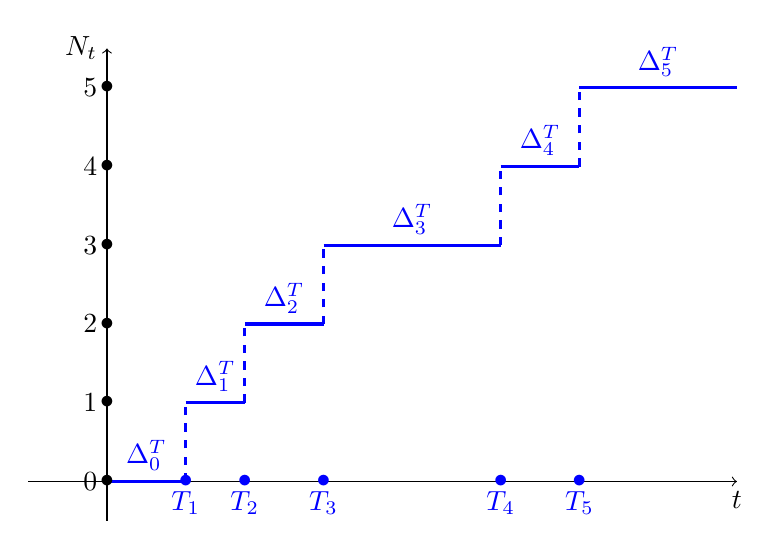
\begin{tikzpicture}[scale=1]
  %Origin and axis
  \coordinate (O) at (0,0);
  \draw[->] (-1,0) -- (8,0) coordinate[label = {below:$t$}] (xmax);
  \draw[->] (0,-0.5) -- (0,5.5) coordinate[label = {left:$N_t$}] (ymax);
  %Lower linear boundary


  %Stochastic process trajectory

  \draw (0,0) node[blue,left] {} node{};
  \draw[very thick,blue,-] (0,0) -- (1,0) node[pos=0.5, above] {$\Delta^T_0$} ;
  \draw[very thick,dashed,blue] (1,0) -- (1,1) node[pos=0.5, right] {};
  \draw[very thick,blue,-] (1,1) -- (1.75,1) node[pos=0.5, above] {$\Delta^T_1$};
  \draw[very thick,dashed,blue] (1.75,1) -- (1.75,2) node[pos=0.5, right] {};
  \draw[very thick,blue,-] (1.75,2) -- (2.75,2) node[pos=0.5, above] {$\Delta^T_2$};
  \draw[very thick,dashed,blue] (2.75,2) -- (2.75,3) node[pos=0.5, right] {};
  \draw[very thick,blue,-] (2.75,3) -- (5,3)node[pos=0.5, above] {$\Delta^T_3$};
  \draw[very thick,dashed,blue] (5,3) -- (5,4) node[pos=0.5, right] {};
  \draw[very thick,blue,-] (5,4) -- (6,4) node[pos=0.5, above] {$\Delta^T_4$};
  \draw[very thick,dashed,blue] (6,4) -- (6,5) node[pos=0.5, right] {};
  \draw[very thick,blue,-] (6,5) -- (8,5) node[pos=0.5, above] {$\Delta^T_5$};
  %Jump Times
  \draw (1,0) node[blue,below] {$T_1$} node{ \color{blue}$\bullet$};
  \draw (1.75,0) node[blue,below] {$T_2$} node{ \color{blue}$\bullet$};
  \draw (2.75,0) node[blue,below] {$T_3$} node{ \color{blue}$\bullet$};
  \draw (5,0) node[blue,below] {$T_4$} node{ \color{blue}$\bullet$};
  \draw (6,0) node[blue,below] {$T_5$} node{ \color{blue}$\bullet$};
  %Level of the counting process
   \draw (0,0) node[black,left] {$0$} node{ \color{black}$\bullet$};
   \draw (0,1) node[black,left] {$1$} node{ \color{black}$\bullet$};
   \draw (0,2) node[black,left] {$2$} node{ \color{black}$\bullet$};
   \draw (0,3) node[black,left] {$3$} node{ \color{black}$\bullet$};
   \draw (0,4) node[black,left] {$4$} node{ \color{black}$\bullet$};
   \draw (0,5) node[black,left] {$5$} node{ \color{black}$\bullet$};
\end{tikzpicture}
\end{center}
\caption{Une trajectoire du processus de comptage $(N_t)_{t\geq0}$.}
\label{fig:trajectory_counting_process}
\end{figure}
\begin{definition}\label{def:exp_dist}
Une \va $X\sim\ExpDist(\lambda)$ est une \va continue de densité
$$
f_X(x) =\lambda\e^{-\lambda x}\ind_{(0,\infty)}.
$$
\end{definition}
\begin{definition}\label{def_poisson_process}
Un processus de Poisson $(N_t)_{t\geq0}$ d'intensité $\lambda$ est un processus de comptage dont les temps inter-arrivée \iid sont de loi exponentielle $\ExpDist(\lambda)$.
\end{definition}
\begin{remark}\label{def_renewal_process}
Le processus de Poisson appartient à la famille des processus de renouvellement qui sont des processus de comptage dont les temps inter-arrivée sont \iid.
\end{remark}
Dans le modèles considéré, l'arrivée des sinistres est modélisée par un processus de Poison $(N_t)_{t\geq0}$ d'intensité $\lambda>0$. Pour chaque sinistre une indemnisation est versée aux assurés. ces indemnisation forment une suite $(U_n)_{n\geq0}$ de \va \iid et positives. Finalement la richesse de la compagnie d'asssurance est donnée par 
\begin{equation}\label{eq:cramer_lundberg_modele}
X_t = x + ct - \sum_{k=1}^{N_t}U_k,\text{ }t\geq 0.
\end{equation}
Usuellement les primes sont reçues à la date d'anniversaire des contrats. Ici, on suppose que le portefeuille est suffisamment important pour pouvoir approcher l'encaissement des primes par une fonction linéaire de pente $c$. La gestion des risque repose souvent sur la définition d'une mesure de risque qui résume par un nombre le risque sous-jacent. En théorie du risque, on utilise la probablité de ruine à un horizon de temps $T\geq 0$ définie par 
$$
\psi(x,T) = \Prob\left(\tau_0^-\leq T\right),
$$
où $\tau_0^- = \inf\{t\geq 0\text{ ; }X_t\leq0\}$ est le premier instant pour lequel la richesse de l'assureur passe en dessous de $0$. L'objectif de l'actuaire est dès lors de déterminer un niveau de prime $c$ et une richesse initiale $x$ associé à un niveau de risque $\psi(x,T) = 1-\alpha$. La directive européenne Solvabilité II impose un niveau de risque $\alpha = 99.5\%$ à horizon de temps $T= 1 \text{an}$. Le niveau de prime compense le cout moyen des sinistre par unité de temps avec 
$$
c = (1+\eta)\frac{1}{t}\E\left(\sum_{k=1}^{N_t}U_k\right) = (1+\eta)\lambda\E(U),
$$
où $\eta>0$ est le chargement de sécurité (de combien la prime commercial ecxcède la prime pure). On définit également la probabilité de ruine ultime par 
$$
\psi(x) = \underset{T\rightarrow \infty}{\lim} \psi(x,T),
$$
nous verrons que si $\eta \leq 0$ alors $\psi(x) = 1$. Une fois le niveau de prime fixé, le seul paramètre à ajusté est le niveau de richesse initiale $x$ dont la détermination passe par l'évaluation numérique de la probabilité de ruine.
\section{Généralités sur les processus en temps continu}\label{sec:processus_continu}
\subsection{Définitions}\label{ssec:definitions}
Soit $(\Omega, \F, \Prob)$ un espace probabilisé. 
\begin{definition}\label{def:filtration}
Une filtration $(\F_t)_{t\geq0}$ est une suite croissante croissante pour l'inclusion avec
$$
\F_s\subset \F_t,\text{ pour }s\leq t,
$$
de sous-tribu de $\F$.
\end{definition}
Soit $(\F_t)_{t\geq0}$ une filtration de $(\Omega, \F, \Prob)$. $\F_t$ correspond à l'information disponible au temps $t$,
\begin{definition}\label{def:processus}
Une suite $(X_t)_{t\in \RL_+}$ de variable aléatoires (\va) sur $\Omega$ est un processus stochastique en temps continu. $X$ est $\F_t$-adapté si $X_t$ est mesurable par rapport à $\F_t$ pour tout $t\geq0$. 
\end{definition}
\begin{remark}
La filtration $\F_t$ associée à un processus $(X_t)_{t\geq 0}$ est l'information qu'il faut détenir pour pouvoir tracer la trajectoire du processus jusqu'à l'instant $t\geq 0$. Pour le processus de comptage, il s'agit des instants de saut 
$$
\F_t = \sigma[T_k\ind_{T_k \leq t})_{k\geq 0}].
$$
Pour le processus de richesse il faut ajouter la taille des sauts
$$
\F_t=\sigma[(T_k\ind_{T_k \leq t}, U_k)_{k\geq 0}].
$$
\end{remark}
% \begin{definition}\label{def:processus_egaux}
% Deux processus $X$ et $Y$ sont égaux en loi, noté $X \overset{\mathcal{D}}{=} Y$, si 
% $$
% (X_{t_1}, \ldots, X_{t_n})\overset{\mathcal{D}}{=} (Y_{t_1}, \ldots, Y_{t_n}),\text{ pour tout } n\in \N\text{ et }(t_1,\ldots, t_n)\in \RL_+^n.
% $$
% \end{definition}
\subsection{Propriétés fonctionnelles}
Soit $\omega\in\Omega$,  est une trajectoire ou réalisation. Il s'agit d'une fonction du temps $t\mapsto X_t(\omega)$ dont on peut étudié les propriétés comme la monotonie, la continuité, et la dérivabilité 
\begin{itemize}
  \item Un processus $X$ est croissant la fonction $t\mapsto X_t$ est croissante presque surement (\ps).
  \item Un processus $X$ est continu à droite, continu, dérivable, de classe $\mathcal{C}^2$, $\ldots$ si  $t\mapsto X_t$ vérifie la propriété considéré.
\end{itemize}
\begin{ex}
Les trajectoires des processus de comptages sont continue à droite et limité à gauche (càdlàg), cela signifie que 
\begin{itemize}
    \item $\underset{s\uparrow t}{\lim}X_s$ existe
    \item $\underset{s\downarrow t}{\lim}X_s$ existe et est telle que $\underset{s\downarrow t}{\lim}X_s = X_t$ 
\end{itemize}
La fitration $\F_{T_{i}}$ jusqu'à un instant de saut $T_i$ implique la continuité juste après le saut. Sinon la trajectoire est continue par morceaux. Même remarque pour le processus de richesse.
\end{ex}
\section{Temps d'arrêt}\label{sec:temps_arret_contd}
Soit $(\Omega,\F, \F_t,\Prob)$ un espace de probabilité filtré.
\begin{definition}
Un temps d'arrêt relativement à $(\F_t)_{t\geq0}$ est une \va à valeur dans $\RL_+\cup\{\infty\}$ telle que 
$$
\{\tau\leq t\}\in\F_t,\text{ pour }t\in\RL_+
$$

\end{definition}
\begin{ex}
\begin{enumerate}
    \item Les constantes sont des temps d'arrêts
    \item Si $\tau$ et $\sigma$ sont des temps d'arrêts alors 
    $$
    \tau\land\sigma, \tau\vee\sigma,\text{ et }\tau + \sigma
    $$
    sont également des temps d'arrêt.
    \item Si $X$ est un processus $\F_t$-adapté, continu à droite et tel que $X_0 = 0$, alors 
    $$
    \tau_a^+ = \inf\{t\geq 0\text{ ; }X_t\geq a\}
    $$
    est un temps d'arrêt. En effet
    \begin{equation}\label{eq:hitting_time}
    \{\tau_a>t\} = \{X_s\leq a\text{ ; }s\leq t\} = \bigcap_{s\in\Q\leq t}\{X_s\geq a\}\in\F_t.
    \end{equation}
    L'hypothèse de continuité à droite est ici primordiale pour définir une suite de rationnelle $s_n\rightarrow s$ tel que $X_{s_n}\rightarrow X_s$ presque sûrement. On passe à la limite \eqref{eq:hitting_time} et la statbilité des tribus par intersection dénombrable permet de conclure.
    \item le temps de dernier passage 
        $$
    T_a = \sup\{t\geq 0\text{ ; }X_t>a\}
    $$
    n'est en général pas un temps d'arrêt.
    \item Le temps de ruine
    $$
    \tau_0^- = \inf\{t\geq 0\text{ ; }X_t\leq 0\}
    $$
    est un temps d'arrêt.
\end{enumerate}
\end{ex}
\begin{prop}
Si $\tau$ et $\sigma$ sont des temps d'arrêt tels que $\sigma<\tau$ alors
$$
\F_\sigma\subset\F_\tau
$$
\end{prop}
\begin{proof}
Soit $A\in\F_\sigma$, montrons que $A\in\F_\tau$. Pour tout $t\geq 0$, on a 
$$
A\cap\{\tau\leq t\} = A\cap\{\tau\leq t\}\cap\{\sigma\leq t\}.
$$
puisque $\sigma\leq \tau$. 
\begin{itemize}
\item $\{\tau\leq t\}\in\F_t$ car $\tau$ est un $\F_t$-temps d'arrêt,
\item $A\cap\{\sigma\leq t\}\in\F_t$ car $\sigma$ est $\F_t$-temps d'arrêt et $A\in\F_\sigma\subset\F_t$
\end{itemize}
On en déduit 
$$
A\cap\{\tau\leq t\}\cap\{\sigma\leq t\}\in\F_t.
$$
\end{proof}
\begin{prop}
Soit $X$ un processus $\F_t$-adapté et continu à droite. Soit $\tau$ un $\F_t$-temps d'arrêt. La \va
$$
X_\tau\ind_{\tau<\infty}\text{ est }\F_\tau\text{-mesurable}.
$$
On rappelle que la \va vérifie $X_\tau(\omega) = X_{\tau(\omega)}(\omega)$
\end{prop}
\section{Martingale}\label{sec:temps_arret_contd}
Soit $(\Omega,\F, \F_t,\Prob)$ un espace de probabilité filtré, et $X$ un processus $\F_t$-adapté.
\begin{definition}\label{def:martingale_contd}
$X$ est une $\F_t$-martingale si 
\begin{itemize}
    \item $\E(|X_t|)<\infty$ pour $t\geq 0$
    \item $\E(X_t|\F_s) = X_s$ pour tout $s\leq t$.
\end{itemize}
\end{definition}
\begin{ex}
Soit $(N_t)_{t\geq 0}$ un processus de Poisson et $(U_i)_{i\geq 0}$ une suite de \va \iid.
\begin{enumerate}
    \item le processus $N_t-\lambda t$ est une martingale
    \item le processus $\sum_{i = 1}^{N_t}U_i-\lambda\E(U) t$ est une martingale
\end{enumerate}
\end{ex}
\begin{definition}
$X$ est une $\F_t$-sous martingale (resp. sur martingale) si 
$$
 \E(X_t|\F_s) \geq\text{ (resp. }\leq) X_s
$$
\end{definition}
Une martingale est un processus constant en moyenne, une sous martingale est un processus croissant en moyenne, et une sur martingale est un processus décroissant en moyenne.
\begin{prop}
Soit $T> 0$ un horizon de temps, si $X$ est une $\F_t-$martingale alors le processus $(X_t)_{t\leq T}$ est complétement déterminé par sa valeur terminale au sens où 
$$
X_t = \E(X_T|\F_t).
$$
\end{prop}
\begin{definition}[martingale fermée]\label{def:closed_martingale}
Une martingale $X$ est fermée, s'il existe $Z\in\mathcal{L}^1
(\Omega,\F, \Prob)$ ($\E(|Z|)<\infty$) telle que 
$$
X_t  =\E(Z|\F_t),\text{ pour tout }t\geq 0
$$

\end{definition}
\begin{definition}[Uniforme intégrabilité]\label{def:UI}
Un processus $X$ est uniformément intégrable si les deux conditions suivantes sont vérifiées
\begin{enumerate}
    \item $\exists M> 0$, tel que $\E|X_t|<M$ pour tout $t\geq 0$
    \item $\forall \epsilon> 0$, $\exists \delta> 0$ tel que $\forall A\in\F$ tel que $\Prob(A)<\delta$, on a $\E\left(|X_t|\ind_A\right)<\epsilon$ pour tout $t\geq $0
\end{enumerate}
\end{definition}
\begin{theo}\label{theo:martingale_convergence}
Soit $X$ une martingale. Les assertions suivantes sont équivalentes:
\begin{enumerate}
    \item $X$ est une martingale fermée
    \item $X$ converge presque sûrement et dans $\mathcal{L}^1$ vers $X_\infty$
    \item $X$ est uniformément intégrable
\end{enumerate}
\end{theo}
\begin{theo}[du temps d'arrêt optionnel Doob]\label{theo:doob_stopping_theorem}
Soient $X$ une $\F_t$-martingale, $\tau$ et $\sigma$ deux temps d'arrêt tel que $\sigma\leq \tau$ \ps. Supposons que $X$ soit UI ou que les temps d'arrêt soient finis \ps. Alors on a 
$$
\E(X_{\tau}|\F_\sigma) = X_\sigma.
$$
En particulier, 
$$
\E(X_{\infty}|\F_\sigma) = X_\sigma.
$$
et 
$$
\E(X_0) = \E(X_{\sigma}) =\E(X_{\infty}).
$$
\end{theo}
\begin{remark}

\begin{enumerate}
    \item Lorsque $X$ n'est pas UI, une technique classique consiste à considérer le temps d'arrêt $\tau\land t$ puis à faire tendre $t$ vers $\infty$
    \item Si la martingale est UI alors elle est fermé par $X_\infty$ et on peut considérer des temps d'arrêt infini. On a 
    $$
    \E(X_\infty|\F_\sigma) = X_\sigma.
    $$
\end{enumerate}
\end{remark}
Pour un exposé plus exhaustif avec notamment toutes les preuves, le lecteur peut consulter l'ouvrage de \citet[Chapitre 3]{Gall2012}\footnote{\url{http://raphaelducatez.neowordpress.fr/wp-content/uploads/sites/20439/2019/02/Jean-Francois_Le_Gall_auth._Mouvement_brownienb-ok.cc_.pdf}}.
\section{Processus de Lévy}\label{sec:levy}
\subsection{Définitions}
L'équivalent des marches aléatoires en temps continu sont les processus de Lévy. Soit $(\Omega,\F,\F_t,\Prob)$ un espace de probabilité filtré et $X$ un processus $\F_t-$adapté.
\begin{definition}
$X$ est un processus de Lévy s'il possède les propriétés suivantes:
\begin{enumerate}
    \item $X_0 = 0$
    \item $X_t - X_s \overset{\mathcal{D}}{=}X_{t-s}\text{ (Accroissements stationaires)}$
    \item Pour tout $n\in\N$ et $0\leq s_1\leq t_1\leq s_2\leq t_2\leq \ldots\leq s_n\leq t_n<\infty$, les accroissements
    $$
    X_{t_i}-X_{s_i},\text{ }i = 1,\ldots, n,
    $$
    sont indépendants.
    \item Les trajectoires de $X$ sont càdlàg
\end{enumerate}
\end{definition}
\begin{ex}
\begin{enumerate}
    \item Le processus de Poisson $N$ est un processus de Lévy avec 
    $$
    N_t - N_s\sim\PoissonDist(\lambda(t-s)),\text{ pour }0\leq s<t<\infty.
    $$
    \item Le processus de poisson composé 
    $$
    \sum_{i = 1}^{N_t}U_i, \text{ }t\geq 0,
    $$
    est un processus de Lévy.
    \item Le processus de richesse
    $$
    ct-\sum_{i = 1}^{N_t}U_i,\text{ }t\geq 0,
    $$
    est un processus de Lévy.
\end{enumerate}
\end{ex}
\begin{remark}
On considère le modèle de Cramer-Lundberg 
$$
X_t = x +ct-\sum_{i = 1}^{N_t}U_i,\text{ }t\geq 0.
$$
Soit $T_1,T_2,\ldots$ les instants de sauts du processus de Poisson et $\Delta T_1,\Delta T_2,\ldots, $ les temps inter-arrivées. Si on observe le processus de richesse aux instants de saut, on définit un processus de richesse à temps discret avec 
$$
Y_n = X_{T_n} = x +cT_n -\sum_{i = 1}^{N_{T_n}}U_i = x +c\sum_{i = 1}^{n}\Delta T_i -\sum_{i = 1}^{n}U_i = x +\sum_{i = 1}^{n}(c\Delta T_i -U_i),\text{ }n\geq 0 .
$$
Il s'agit d'un marche aléatoire, identique à celle étudié dans la \cref{sec:ruin_discret}.
\end{remark}
Soit $X$ un processus de Lévy.
\begin{definition}
L'exposant de Laplace de $X$ est défini par 
$$
\kappa(\theta) = \log \E(\e^{\theta X_1}).
$$
\end{definition}
Il s'agit de la fonction génératrice des cumulants de $X_1$.
\begin{ex}
L'exposant de Laplace du processus de Poisson $N$ d'intensité $\lambda$ est donnée par 
$$
\kappa(\theta) = \log\E(\e^{\theta N_1}) = \lambda(\e^\theta - 1). 
$$
\end{ex}
\begin{prop}
On a 
$$
\log \E(\e^{\theta X_t}) = \kappa(\theta)t,\text{ pour tout }t\geq 0
$$
\end{prop}
\begin{proof}
Soit $t\geq 0$ et $n\in \N$, on décompose $X_t$ avec 
$$
X_t=\sum_{k=0}^{n-1}\left(X_{(k+1)\frac{t}{n}} - X_{k\frac{t}{n}} \right).
$$
On a 
\begin{eqnarray*}
\E\left(e^{\theta X_t}\right)&=&\E\left(e^{\theta \sum_{k=0}^{n-1}\left(X_{(k+1)\frac{t}{n}} - X_{k\frac{t}{n}} \right)}\right)\\
&=&\prod_{k=0}^{n-1}\E\left(e^{\theta \left(X_{(k+1)\frac{t}{n}} - X_{k\frac{t}{n}} \right)}\right)\\
&=&\prod_{k=0}^{n-1}\E\left(e^{\theta X_{t/n}}\right)\\
&=&\E\left(e^{\theta X_{t/n}}\right)^n\\
\end{eqnarray*}
Si on note 
$$
\kappa_t(\theta) = \log \E\left(e^{\theta X_t}\right)
$$
On a donc $\forall t\geq 0$ et $\forall n\in \N$,
$$
\kappa_t(\theta) = n\kappa_{t/n}(\theta).
$$
De plus pour $m\in\N$, on a 
$$
\kappa_m(\theta) = m\kappa(\theta)\text{ et }\kappa_m(\theta) = n\kappa_{m/n}(\theta).
$$
On en déduit que 
$$
\kappa_t(\theta) = t\kappa(\theta)\text{ pour }t\in\Q
$$
On peut alors considérer une suite $(t_n)_{n\geq 0}\in \Q$ tel que $t_n\downarrow t\in \RL$ puis passer à la limite 
$$
\kappa_{t_n}(\theta) = t_n\kappa(\theta)\text{ pour }t\in\Q.
$$
Tout cela est possible grâce à la continuité à droite des trajectoires du processus.
\end{proof}
\begin{prop}[Martingale de Wald]\label{prop:Wald_martingale_Levy}
Le processus 
$$
M_t = \exp\left[\theta X_t - t\kappa(\theta)\right],\text{ }t\geq 0.
$$
est une $\F_t$-martingale.
\end{prop}
\begin{proof}
soit $s\leq t$, On a 
\begin{eqnarray*}
\E(M_t|\F_s)&=&\e^{-t\kappa(\theta)}\E\left[\e^{\theta X_t}|\F_s\right]\\
&=&\e^{-t\kappa(\theta)}\E\left[\e^{\theta (X_t-X_s) +\theta X_s}|\F_s\right]\\
&=&\e^{-t\kappa(\theta)}\e^{\theta X_s}\E\left[\e^{\theta (X_t-X_s)}\right]\\
&=&\e^{-t\kappa(\theta)}\e^{\theta X_s}\e^{(t-s)\kappa(\theta)}\\
&=&M_s\\
\end{eqnarray*}
\end{proof}
Cette martingale est très pratique pour résoudre des problèmes de premier passage pour des processus de Lévy, conjointement avec la propriété de Markov forte.
\begin{theo}\label{theo:levy_strong_markov}
Soit $\tau$ un temps d'arrêt tel que $\tau<\infty$ presque sûrement. Le processus $\tilde{X}$ défini par 
$$
\tilde{X}_t = X_{\tau + t}-X_{\tau},t\geq 0,
$$
est un processus de Lévy indépendant de $\F_\tau$ de même loi que $X$.
\end{theo}
\begin{proof}
Admis, voir \citet[Chapitre 3]{Kyprianou2014}
\end{proof}

L'étude de temps de premier passage est centrale en théorie du risque et est l'objet de la théorie de la fluctuation. Pour une vue exhaustive, le lecteur peut consulter l'ouvrage de \citet{Kyprianou2014}\footnote{\url{https://people.bath.ac.uk/ak257/book2e/book2e.pdf}}. Nous nous focalisons dans la section suivante sur le processus de Cramer Lundberg.
\subsection{Application à l'étude du processus de Cramer-Lundberg}
On considère le processus 
$$
X_t = x +ct - \sum_{i = 1}^{N_t}U_i.
$$
Soit 
$$
\tau_0^- = \inf\{t\geq 0\text{ ; }X_t\leq 0\},
$$
le temps de ruine. 
\begin{prop}
Si $c\leq \lambda\E(U)$ alors 
$$
\psi(u) = \Prob(\tau_0^-<\infty)=1.
$$
\end{prop}
\begin{proof}
On note que 
$$
\underset{t\rightarrow \infty}{\lim} \frac{X_t}{t}= \underset{t\rightarrow \infty}{\lim}\left(\frac{x}{t}+c-\frac{N_t}{t}\frac{\sum_{i=1}^{N_t}U_i}{N_t}\right) = c-\lambda \E(U),
$$
et donc 
$$
\underset{ t\rightarrow \infty}{\lim} \frac{X_t}{t} = \begin{cases}
+\infty,&\text{ si }c-\lambda \E(U)>0,\\
?,&\text{ si }c-\lambda \E(U)=0,\\
-\infty,&\text{ si }c-\lambda \E(U)<0.
\end{cases}
$$
Pour le cas $c-\lambda \E(U)=0$, il faut considérer la marche aléatoire $Z_n = X_{T_n}$ qui est récurrente, ce qui implique que l'état $0$ est récurrent et donc $\psi(u) =1$.
\end{proof}
Le résultat suivant donne une borne superieur pour la probabilité de ruine. 
\begin{theo}
Supposons que $c>\lambda\E(U)$ alors 
$$
\psi(x) =  \frac{ \e^{-\theta^\ast x}}{\E\left[\e^{\theta^\ast d(x)}|\tau_0^-<\infty\right]},
$$
où $\theta^\ast$ est la seule solution strictement positive de l'équation 
$$
-\theta c + \lambda [\E(\e^{\theta U})-1] = 0,
$$
et $d(x) = -X_{\tau_0^-}$ est le définit à la ruine. 
\end{theo}
\begin{proof}
Le processus $Y$ défini par
$$
Y_t = x - X_t = \sum_{i=1}^{N_t}U_i - ct,\text{ }t\geq 0,
$$
est un processus de Lévy d'exposant de Laplace 
$$
\kappa(\theta) = -c\theta+\lambda\left[\E(\e^{\theta U})-1\right].
$$
On note que $\underset{\theta\rightarrow \infty}{\lim}\kappa(\theta) = \infty$, $\kappa(0) = 0$ et $\kappa'(0) = \lambda\E(U)-c<0$. Cela implique que l'équation 
$$
\kappa(\theta)=0
$$
a une unique solution strictement positive $\theta^\ast$. Le processus $\left(\e^{\theta^\ast Y_t}\right)_{t\geq 0}$ est une martingale en vertu de la \cref{prop:Wald_martingale_Levy}. On applique le théorème du temps d'arrêt optionnel au temps d'arrêt $\tau_0^-\land t$ pour $t\geq 0$. Il vient 
\begin{eqnarray*}
1&=&\E\left(\e^{\theta^\ast Y_0}\right)\\
&=&\E\left(\e^{\theta^\ast Y_{\tau_0^-\land t}}\right)\\
&=&\E\left(\e^{\theta^\ast Y_{\tau_0^-}}\ind_{t>\tau_0^-}+\e^{\theta^\ast Y_{t}}\ind_{t\leq \tau_0^-}\right)\\
\end{eqnarray*}
On fait tendre $t$ vers $+\infty$ pour obtenir
$$
1 = \E\left(\e^{\theta^\ast Y_{\tau_0^-}}|\tau_0^-<\infty\right)\Prob(\tau_0^-<\infty)=\e^{\theta^\ast x}\E\left(\e^{-\theta^\ast X_{\tau_0^-}}|\tau_0^-<\infty\right)\psi(x)
$$
ce qui est équivalent à 
$$
\psi(x)=\frac{\e^{-\theta^\ast x}}{\E\left(\e^{-\theta^\ast X_{\tau_0^-}}|\tau_0^-<\infty\right)}.
$$

\end{proof}
Il s'agit d'un résultat fondateur de théorie de la ruine, voir l'ouvrage de référence de \citet{Asmussen2010} et l'application de la théorie de la fluctuation au processus de Cramer-Lundberg, voir \citet{Kyprianou2013}\footnote{\url{https://people.bath.ac.uk/ak257/GSZurich-Guanajuato.pdf}}. 
\newpage